\chapter{绪论}

\section{研究背景和意义}
检索任务的定义是指根据用户特定的信息需求,对这种特定的信息采用一定的方
法、技术手段,根据一定的线索与规则找到满足用户需求的信息。同款服装检索作为检
索的子任务,则是需要根据用户提供的需求信息,在由多种款式、风格的服装图片组成
的检索库中找到其同款服装。

几年前,网页购物的快速便捷极大的促进了人们消费水平的进步,随后,各大电商
平台进一步将它们的购物应用推广到了用户的手机里。也正是因为这样,用户的购买习
惯也在悄悄地发生着改变:时间和地点不再是局限,只要拥有一部连接互联网的手机,
就可以直接获取想要购买的商品。随着移动技术的迅速发展,移动设备的安全、高速、
便捷等特点越来越获得人们的认可,这就使得移动购物的行为变得越来越普遍。然而目
前 PC 和移动终端中,用户多数情况下还是通过输入文本关键词以获取目标商品,用这
种单一的文本信息去描述商品有时很难表达用户的真实需求。

这种基于文本信息的由粗到精的检索方式,一定程度上可以帮助用户定位到有具体
标签的商品。然而,当用户需求的商品的一些关键信息不明确时,抽象出适合的关键词
去进行检索就变得很困难了,这种情况下以图搜图的检索方式能更好的表达用户的需
求。CBIR (Content-Based Image Retrieval)\cite{kato1992sketch},即基于内容的图像检索, 是近十年来计算机
视觉最关注的研究领域之一, CBIR 是通过分析提取图像的视觉或语义特征, 使用相似度
度量算法, 从检索库中得到一组与其最为相似的图像。从根本上来讲,CBIR 是一种相似
度度量技术, 它包含了图像处理、计算机视觉和图像理解等领域,是国内外研究的热点。

如今,各大电商平台已经提供了以图搜图的功能,消费者可以上传实时照片以检索
同款商品,如图\ref{fig:tb}所示。随着互联网及多媒体技术的迅速发展, 图像的来源不断扩大,
高速、大容量的存储系统为存储海量图像提供了保障,图像信息在各行各业都越来越广
泛的被使用, 因此,图像信息资源的高效管理和高性能的检索算法变得日益重要。图像
检索是图像数据研究的一项核心技术, 是近年来海量信息处理所面临的“瓶颈”。所以,
对基于图像内容的检索算法的研究有重要意义。
\begin{figure*}[h]
  \centering
  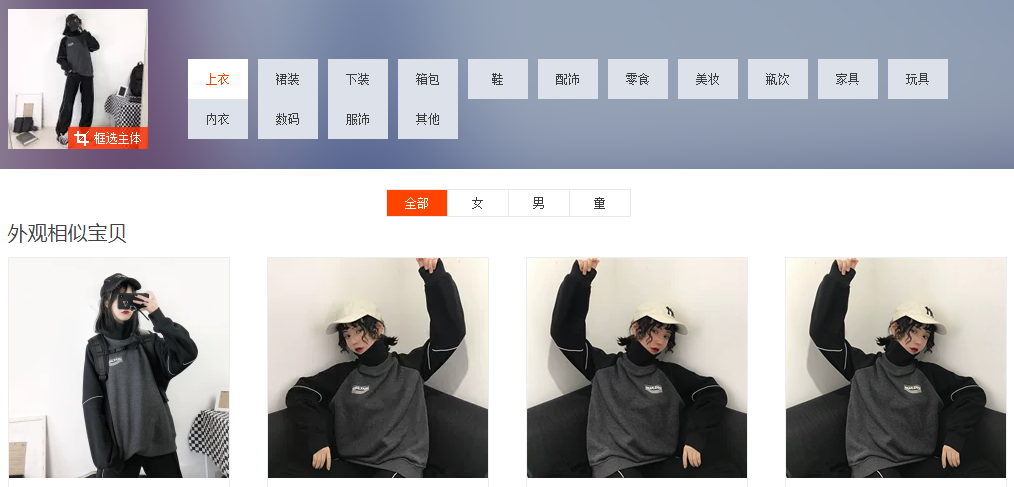
\includegraphics[width = 1\linewidth]{Img/tb.png}
  \caption{淘宝提供的以图搜图功能,用于检索同款商品}
  \label{fig:tb}
\end{figure*}


\section{研究内容及贡献}
本课题采用 DeepFashion\cite{liu2016deepfashion} 数据集作为训练集,阿里巴巴 2017 大规模图像搜索大赛
的数据集作为测试集,共 300 万张测试图片。评价标准为上装,裙装和下装的检索 top4
命中率,对应的目标性能分别为 85\%、80\%、75\%。

对于服装图像检索这项任务,局部特征的学习与对齐一直是研究的重要方向,这也
是本课题面临的最大考验。此外,深度学习一直以来都有一个问题:训练好的模型在另
外一个域的性能会下降。基于这些问题,本课题的研究内容主要针对如下内容展开:(1)
探究度量学习以及多任务学习,以提升模型表达能力;(2)研究模型在不同域数据集
之间性能不一致的问题,提升模型泛化能力;(3)探索如何有效结合局部特征以及全局
特征,以及更加准确的局部区域对齐方式。据此,本文的主要贡献有如下几个方面:
\begin{itemize}
  \item [1.] 引入注意力机制,让网络自适应的学习应该重点关注的局部区域。学习特征空间维度的权重分布,弱化图像中的噪音部分,且网络训练过程中除了类别标签外不需要额外的
    标注信息。采用多个分支并行的架构,可以使得每个分支关注的局部区域有所区别,进一步提升模型的表达能力。

  \item [2.] 提出跨域样本挖掘的方法。模型在实际使用场景下的输入数据与训练数据集常常有一定的区别,这种情况之下模型的性能往往达不到预期,因为来自不同域的数据集的数据
    分布与训练集本身就有差别。基于此,本文提出一种跨域挖掘样本的方式:先在原有的训练集训练出一个模型,然后在不同域的测试集中随机选择一定量的图像作为模型输入
    并在测试集做检索,每张输入图像都会得到Top K的排序输出,我们取这K张图片中排序相对靠前的图像作为和输入图像的同款服装样本,排序靠后的作为非同款样本,最后把这些样本
    放入原有的训练集训练。通过这种方式,模型可以更好的适应测试集的数据分布,进而有效提升在测试集的表现。
  
  \item [3.] 提出多粒度切分的方法,大幅度增强特征的局部表达能力。分类任务一般基于整幅图的全局特征去做,本文在保留全局特征分类做法的基础上,增加了局部特征分类的分支,
    采用切分的方式,对特征图切分为N等份,每一块局部特征经过Average Pooling之后用类别标签去做监督。另外,使用不同大小的N作切分,多粒度的切分分支并行训练,进一步提升模型的性能。

  \item [4.] 提出环形Pooling的策略。首先通过环形的切分方式,得到环形的特征块,对每快特征做环形的平均池化,可以有效解决实际场景常见的旋转问题,结合横向切分和纵向切分,
    使得网络对局部特征的学习更加全面。

\end{itemize}

